\subsection{Application on random images}
In this section we show result for applying unsupervised Convolutional Sparse Coding (denoted as CSC) presented before on 7 random images, 6 for our train and 1 for our test.
\begin{figure}[h]
 \centering
 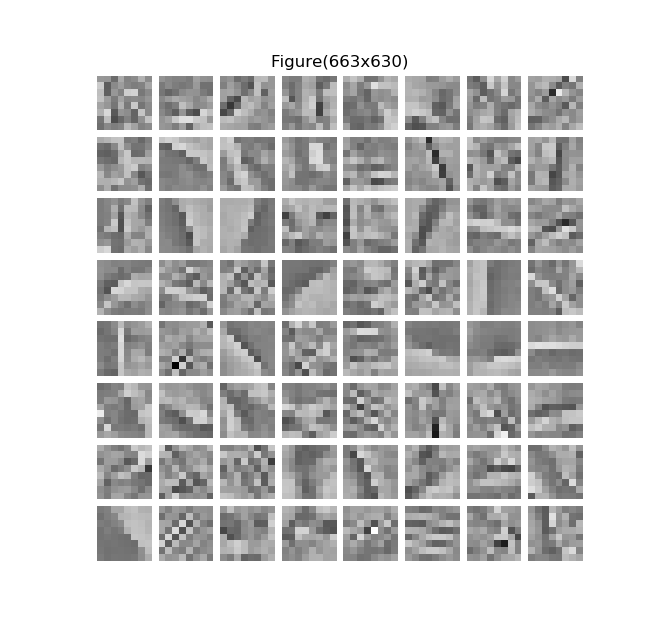
\includegraphics[scale=0.6]{../Results/SPORCO_test_img/Figure_2.png}
 % Figure_2.png: 663x630 px, 100dpi, 16.84x16.00 cm, bb=0 0 477 454
 \caption{Dictionary learned with 6 random images}
\end{figure}
\begin{figure}[h]
 \centering
 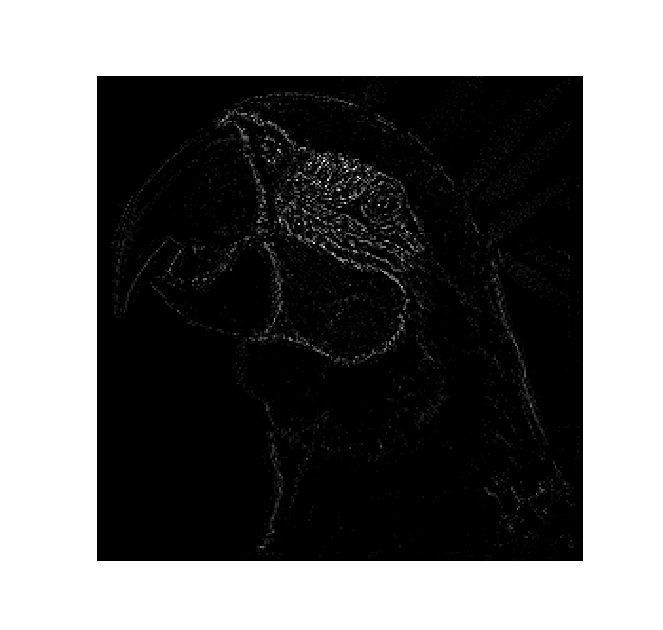
\includegraphics[scale=0.455]{../Results/SPORCO_test_img/activations.png}
 % activations.png: 663x630 px, 100dpi, 16.84x16.00 cm, bb=0 0 477 454
 \caption{Activation}
\end{figure}
\begin{figure}[h]
 \centering
 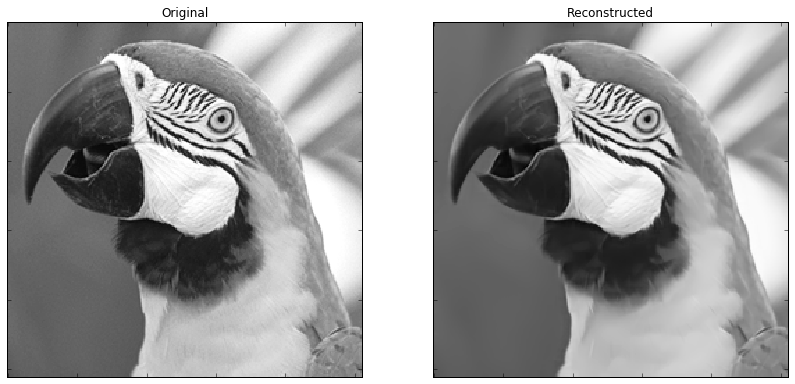
\includegraphics[scale=0.4]{../Results/SPORCO_test_img/recons.png}
 % recons.png: 795x384 px, 72dpi, 28.05x13.55 cm, bb=0 0 795 384
 \caption{Original image vs Reconstructed one}
\end{figure}

